\documentclass{beamer}
\usepackage{fancybox}
\usepackage{tikz}
\usetikzlibrary{arrows.meta,
                chains,
                positioning, 
                shadows.blur, shapes.arrows}

\usepackage{amsmath}              
\usepackage{mathabx}

\usetheme{Madrid}
\newcommand{\G}{\mathcal{G}}

\title{Logic Tensor Networks}

\author{Robert Hoehndorf}
\date{\today}

\begin{document}

\frame{\titlepage}

\begin{frame}
  \frametitle{Introduction}
  \begin{itemize}
  \item Logic Tensor Networks (LTN) is neuro-symbolic framework based
    on fuzzy differentiable logic
  \item Supports tasks based on manipulating data and knowledge
  \item It has been shown to effectively tackle many tasks that are
    central to intelligent systems:
    \begin{itemize}
    \item multi-label classification,
    \item relational learning,
    \item data clustering,
    \item semi-supervised learning,
    \item regression,
    \item embedding learning, and
    \item query answering under uncertainty
    \end{itemize}
  \end{itemize}
\end{frame}

\begin{frame}
  \frametitle{Introduction}
  \begin{itemize}
  \item use of infinitely-valued fuzzy logic (Real Logic)
  \item domains are interpreted as tensors in the Real field
  \item use ``grounding'' instead of ``interpretation''
  \end{itemize}
\end{frame}

\begin{frame}
\frametitle{Real Logic in Logic Tensor Networks}
\begin{itemize}
    \item Real Logic is based on a first-order language \( L \)
    \item Includes constant symbols (\( C \)), functional symbols (\(
      F \)), relational symbols (predicates, \( P \)), and variable
      symbols (\( X \))
    \item Facilitates the expression of relational knowledge with variables
      \begin{itemize}
      \item first order logic
      \end{itemize}
\end{itemize}
\end{frame}

\begin{frame}
\frametitle{Atomic Formulas and Fuzzy Semantics}
\begin{itemize}
    \item Atomic formula example: \( \text{is\_friend}(v1, v2) \)
    \item Symmetric relations example: \( \forall x \forall y
      (\text{is\_friend}(x, y) \Rightarrow \text{is\_friend}(y, x))
      \)
    \item Incorporates fuzzy semantics for partial truth in real-world
      scenarios
\end{itemize}
\end{frame}

\begin{frame}
\frametitle{Types and Domain Assignment}
\begin{itemize}
    \item Domains assigned using functions \( D, D_{in}, \) and \( D_{out} \)
    \item \( D \): Assigns domains to variables and constants
    \item \( D_{in} \) and \( D_{out} \): Define input and output domains
      for functions and predicates
\end{itemize}
\end{frame}

\begin{frame}
\frametitle{Terms and Formulas in Real Logic}
\begin{itemize}
    \item Terms formed from constants, variables, and function symbols
    \item Formulas include atomic formulas, expressions with
      connectives, and quantified expressions
    \item Supports negation, conjunction, disjunction, implication,
      and biconditional, as well as universal and existential
      quantifiers
\end{itemize}
\end{frame}

\begin{frame}
\frametitle{Example of Real Logic Application}
\begin{itemize}
    \item Domains (types): \( \text{Town} \) and \( \text{People} \)
    \item Constants like Alice, Bob (People) and Rome, Seoul (Town)
    \item Example of well-formed expression: \(
      \text{lives\_in}(\text{Alice}, \text{Rome}) \) 
    \item Example of malformed expression: \(
      \text{lives\_in}(\text{Bob}, \text{Charlie}) \)
\end{itemize}
\end{frame}

\begin{frame}
  \frametitle{Semantics}
  \begin{itemize}
  \item Domains are interpreted concretely by tensors in the Real
    field
  \item tensors are algebraic objects that include
    \begin{itemize}
    \item Scalars: 0-dimensional
    \item Vectors: 1-dimensional,
    \item Matrices: 2-dimensional,
    \item as well as higher-dimension structures
    \end{itemize}
  \item To emphasize this, the authors use the term ``grounding'',
    denoted with the letter $\G$, instead of
    ``interpretation'' (the usual name for this concept in logic)
  \end{itemize}
\end{frame}

\begin{frame}
  \frametitle{Semantics}
  Grounding $\mathcal{G}$ maps
  \begin{itemize}
  \item Terms to tensors of real numbers
  \item Formulas to real numbers in the interval [0,1]
  \end{itemize}
\end{frame}

\begin{frame}
  \frametitle{Variables and constants}
  \begin{itemize}
  \item Constants:
    \begin{itemize}
    \item Denote individuals from a space of tensors of any rank:
    \item The individual can be pre-defined (data point) or learnable
      (embedding)
    \item Intuition: Each dimension corresponds to a feature, and the
      number corresponds to the value of that feature for that
      individual
    \end{itemize}
  \item Variables denote sequences of individuals:
    \begin{itemize}
    \item Sequences represent the possible values that the variable can take
    \item They can contain more than one instance of the same value
    \end{itemize}
  \end{itemize}
\end{frame}

\begin{frame}
\frametitle{Functions}
\begin{itemize}
    \item Functions can be any mathematical function, either
      pre-defined or learnable
    \item Examples of functions include distance functions,
      regressors, etc.
\end{itemize}
\end{frame}

% Slide 2: Predicates
\begin{frame}
\frametitle{Predicates}
\begin{itemize}
    \item Represented as mathematical functions mapping an n-ary
      domain of individuals to a real number in \([0,1]\), interpreted
      as a truth degree
    \item Examples of predicates include similarity measures,
      classifiers, etc.
\end{itemize}
\end{frame}

% Slide: Definition 2
\begin{frame}
\frametitle{Definition 2: Grounding in Real Logic}
\begin{block}{Grounding \( \G \) of \( L \)}
A grounding $\G$ of \( L \) is a function defined on the signature of \( L \) that satisfies the following conditions:
\begin{enumerate}
    \item \( \G(x) = \langle d_1, \ldots, d_k \rangle \in
      \bigtimes_{i=1}^{k} G(D(x)) \) for every variable symbol \( x
      \in X \), with \( k \in \mathbb{N}_0 \). \( \G(x) \) is a
      sequence, not a set, allowing multiple occurrences of the same
      value from \( \G(D(x)) \)
    \item \( \G(f) \in \G(D_{\text{in}}(f)) \rightarrow
      \G(D_{\text{out}}(f)) \) for every function symbol \( f \in F
      \)
    \item \( \G(p) \in \G(D_{\text{in}}(p)) \rightarrow [0, 1] \) for
      every predicate symbol \( p \in P \)
\end{enumerate}
\end{block}
\end{frame}

\begin{frame}
  \frametitle{Example}
  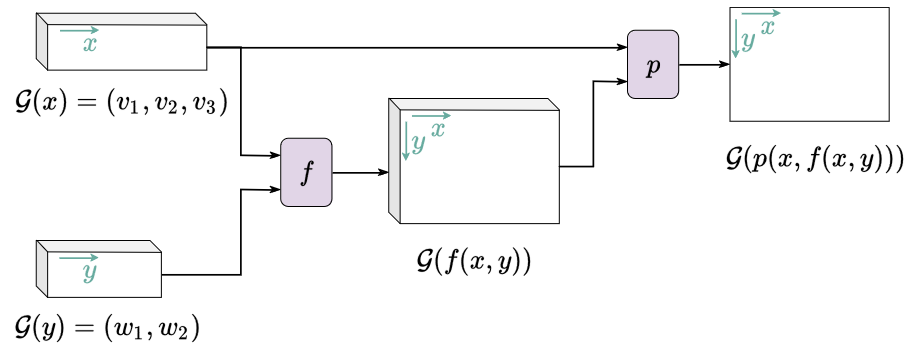
\includegraphics[width=\textwidth]{ltn1.png}
  % Page 7 of LTN Arxiv paper, Example 3
\end{frame}

\begin{frame}
  \frametitle{Connectives}
  Connectives are modeled using fuzzy semantics:
  \begin{itemize}
  \item conjunction: t-norm
  \item disjunction: t-conorm
  \item negation: fuzzy negator
  \item implication: fuzzy implication
  \end{itemize}
  Quantifiers are defined using aggregators (symmetric and continuous
  operators)
  \begin{itemize}
  \item Existential ($\exists$): Generalization of existential quantification in FOL
  \item Universal ($\forall$): Generalization of universal quantification in FOL
  \end{itemize}
\end{frame}

% Slide 1: Table 1 - The t-norms of interest
\begin{frame}
\frametitle{Table 1: The t-norms of Interest}
\resizebox{\textwidth}{!}{
\begin{tabular}{l|l|l}
\textbf{Name} & \textbf{T-norm} & \textbf{Properties} \\
\hline
Gödel (minimum) & \(T_G(a, b) = \min(a, b)\) & idempotent, continuous \\
Product & \(T_P(a, b) = a \cdot b\) & strict \\
Łukasiewicz & \(T_{LK}(a, b) = \max(a + b - 1, 0)\) & continuous \\
Drastic product & \(T_D(a, b) = 
\begin{cases}
\min(a, b), & \text{if } a = 1 \text{ or } b = 1 \\
0, & \text{otherwise}
\end{cases}\) &  \\
Nilpotent minimum & \(T_{nM}(a, b) = 
\begin{cases}
0, & \text{if } a + b \leq 1 \\
\min(a, b), & \text{otherwise}
\end{cases}\) & left-continuous \\
Yager & \(T_Y(a, b) = \max(1 - ((1 - a)^p + (1 - b)^p)^{\frac{1}{p}}, 0), p \geq 1\) & continuous \\
\end{tabular}
}
\end{frame}

% Slide 2: Table 2 - The t-conorms of interest
\begin{frame}
\frametitle{Table 2: The t-conorms of Interest}
\resizebox{\textwidth}{!}{
\begin{tabular}{l|l|l}
\textbf{Name} & \textbf{T-conorm} & \textbf{Properties} \\
\hline
Gödel (maximum) & \(S_G(a, b) = \max(a, b)\) & idempotent, continuous \\
Product (probabilistic sum) & \(S_P(a, b) = a + b - a \cdot b\) & strict \\
Łukasiewicz & \(S_{LK}(a, b) = \min(a + b, 1)\) & continuous \\
Drastic sum & \(S_D(a, b) = 
\begin{cases}
\max(a, b), & \text{if } a = 0 \text{ or } b = 0 \\
1, & \text{otherwise}
\end{cases}\) &  \\
Nilpotent maximum & \(S_{nM}(a, b) = 
\begin{cases}
1, & \text{if } a + b \geq 1 \\
\max(a, b), & \text{otherwise}
\end{cases}\) & right-continuous \\
Yager & \(S_Y(a, b) = \min((a^p + b^p)^{\frac{1}{p}}, 1), p \geq 1\) & continuous \\
\end{tabular}
}
\end{frame}

% Slide: Common Aggregation Operators
\begin{frame}
\frametitle{Common Aggregation Operators}
\resizebox{\textwidth}{!}{%
\begin{tabular}{|l|l|l|}
\hline
\textbf{Name} & \textbf{Generalizes} & \textbf{Aggregation Operator} \\
\hline
Minimum & \( T_G \) & \( A_{T_G}(x_1, \ldots, x_n) = \min(x_1, \ldots, x_n) \) \\
\hline
Product & \( T_P \) & \( A_{T_P}(x_1, \ldots, x_n) = \prod_{i=1}^{n} x_i \) \\
\hline
Łukasiewicz & \( T_{LK} \) & \( A_{T_{LK}}(x_1, \ldots, x_n) = \max\left(\sum_{i=1}^{n} x_i - (n - 1), 0\right) \) \\
\hline
Maximum & \( S_G \) & \( E_{S_G}(x_1, \ldots, x_n) = \max(x_1, \ldots, x_n) \) \\
\hline
Probabilistic sum & \( S_G \) & \( E_{S_P}(x_1, \ldots, x_n) = 1 - \prod_{i=1}^{n} (1 - x_i) \) \\
\hline
Bounded sum & \( S_{LK} \) & \( E_{S_{LK}}(x_1, \ldots, x_n) = \min \left(\sum_{i=1}^{n} x_i, 1\right) \) \\
\hline
\end{tabular}
}
\end{frame}

% Slide 1: Explanation of Types of Implication (S and R)
\begin{frame}
\frametitle{Types of Fuzzy Implications}
Fuzzy implications are functions \( I: [0, 1]^2 \to [0, 1] \) that are increasing with respect to the first argument and decreasing with respect to the second. They satisfy boundary conditions \( I(0, 0) = I(1, 1) = 1 \), and \( I(1, 0) = 0 \). Two classes of fuzzy implications are considered:
\begin{itemize}
    \item \textbf{S-implications}: Formed using a t-conorm and generalizing the material implication \( a \to c = \neg a \oplus c \).
    \item \textbf{R-implications}: Standard in t-norm fuzzy logics,
      constructed from t-norms, $p \rightarrow q \equiv sup\{ t \in [0,1]
      | p \land t \leq q\}$ (or $\max\{ t \in [0,1] | p \land t \leq q\}$)
\end{itemize}
\end{frame}

% Slide: S-implications
\begin{frame}
\frametitle{S-implications with Common t-Conorms}
\resizebox{\textwidth}{!}{%
\begin{tabular}{|l|l|l|l|}
\hline
\textbf{Name} & \textbf{T-conorm} & \textbf{S-implication} & \textbf{Properties} \\
\hline
Gödel (Kleene-Dienes) & \( S_G \) & \( I_{KD}(a, c) = \max(1 - a, c) \) & All but IP \\
Product (Reichenbach) & \( S_P \) & \( I_{RC}(a, c) = 1 - a + a \cdot c \) & All but IP \\
Łukasiewicz & \( S_{LK} \) & \( I_{LK}(a, c) = \min(1 - a + c, 1) \) & All \\
Dubouis-Prade & \( S_D \) & $I_{DP}(a, c) = 
\begin{cases} 
c, & \text{if } a = 1 \\
1 - a, & \text{if } c = 0 \\
1, & \text{otherwise}
\end{cases}$ & All \\
Nilpotent (Fodor) & \( S_{Nm} \) & $I_{FD}(a, c) = 
\begin{cases} 
1, & \text{if } a \leq c \\
\max(1 - a, c), & \text{otherwise}
\end{cases}$ & All \\
\hline
\end{tabular}%
}
\end{frame}

% Slide: Negators and De Morgan Triplets
\begin{frame}
\frametitle{Negators and De Morgan Triplets}
\begin{block}{Negator}
A negator \( n: [0, 1] \to [0, 1] \) is a monotonically decreasing mapping such that \( n(0) = 1 \) and \( n(1) = 0 \). It is:
\begin{itemize}
    \item Strict if it is strictly monotonically decreasing.
    \item Strong if it is strict and involutive, i.e., \( n(n(x)) = x \) for all \( x \in [0, 1] \).
\end{itemize}
The standard (canonical) negator is \( n(x) = 1 - x \), which is both strict and strong.
\end{block}

\begin{block}{De Morgan Triplet}
A De Morgan triplet is a triple \( (T, \perp, n) \) where:
\begin{itemize}
    \item \( T \) is a t-norm.
    \item \( \perp \) is a t-conorm according to the axiomatic definition of t-conorms.
    \item \( n \) is a strong negator.
    \item \( \forall a, b \in [0, 1] \): \( n(\perp(a, b)) = T(n(a), n(b)) \).
\end{itemize}
\end{block}
\end{frame}

\begin{frame}
  \frametitle{Conjunction}
  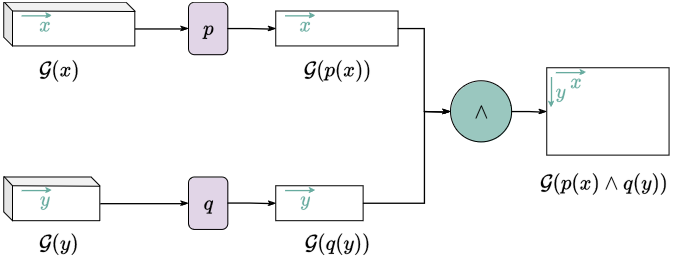
\includegraphics[width=\textwidth]{ltn2.png}
\end{frame}

\begin{frame}
  \frametitle{Quantification}
  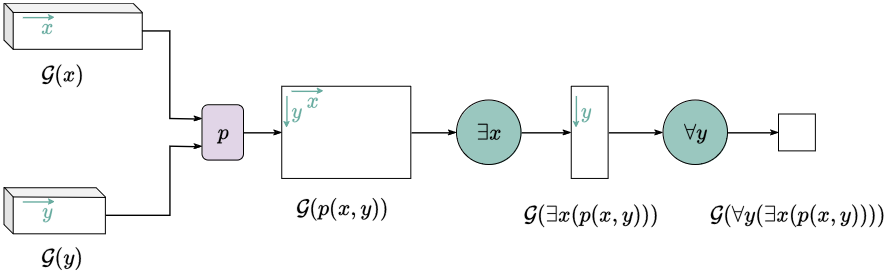
\includegraphics[width=\textwidth]{ltn3.png}
\end{frame}

\begin{frame}
  \frametitle{Operators and Satisfaction Interpretation}
  \begin{block}{Approximating Universal Quantification}
    The operator \( A_{pME} (a_1, \ldots, a_n) \) $=\(
    \frac{1}{n}\sum_{i=1}^n a_i^p \)^\frac{1}{p} $ approximates
    universal quantification as a smooth minimum, influenced by a
    hyper-parameter \( p \) (the exponent in the generalized mean):
    \begin{itemize}
    \item If \( p = 1 \), \( A_{pME} \) corresponds to the
      arithmetic mean.
    \item As \( p \) increases, \( A_{pME} \) converges to the
      min operator, making the quantified formula stricter.
    \end{itemize}
  \end{block}

  \begin{block}{Interpreting Universal Quantification}
    \begin{itemize}
    \item Different values of \( p \) allow for different
      interpretations of universal quantification in propositions:
    \item A low \( p \) value implies that the proposition holds for some \( x \).
    \item A high \( p \) value suggests that the proposition holds for most \( x \).
    \end{itemize}
  \end{block}
\end{frame}

% Slide: Diagonal Quantification in LTN
\begin{frame}
\frametitle{Diagonal Quantification in LTN}
\begin{block}{Diagonal Quantification (Diag)}
\begin{itemize}
    \item Diagonal quantification is denoted as \( \text{Diag}(x_1, \ldots, x_h) \).
    \item It quantifies over specific tuples such that the \( i \)-th tuple contains the \( i \)-th instance of each variable.
    \item Assumes all variables are grounded onto sequences with the same number of instances.
    \item Quantifies over the diagonal of \( G(\phi) \) along the axes associated with \( x_1 \ldots x_h \).
    \item Used for statements that hold true for each pair of sample and label, e.g., \( \forall\text{Diag}(x, y) p(x, y) \) for datasets with samples \( x \) and target labels \( y \).
    \item Reduces computational complexity by avoiding evaluation for all combinations in \( G(x) \) and \( G(y) \).
\end{itemize}
\end{block}
\end{frame}

\begin{frame}
  \frametitle{Diagonal quantification}
  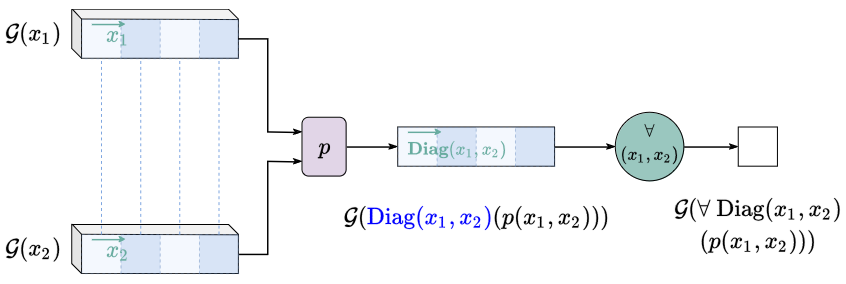
\includegraphics[width=\textwidth]{ltn4.png}
\end{frame}

% Slide: Quantification Over Domain Elements
\begin{frame}
\frametitle{Guarded quantification}
\begin{block}{Quantifying Based on a Condition}
In many situations, it's desirable to quantify over a set of elements
in a domain whose grounding satisfies a specific condition. For
example, one might express a condition using formulas like:
\begin{itemize}
    \item \( \forall y (\exists x : \text{age}(x) > \text{age}(y)) (\text{parent}(x, y)) \)
\end{itemize}
This formula aggregates values of the \textit{parent} predicate only for instances of \( x \) that satisfy the age condition with respect to \( y \).
\end{block}
\end{frame}

% Slide: Grounding Formulas with Conditional Aggregation
\begin{frame}
\frametitle{Grounding Formulas with Conditional Aggregation}
\begin{block}{Aggregating Values Based on Conditions}
The grounding of a formula like \( \forall y (\exists x: \text{age}(x) > \text{age}(y)) (\text{parent}(x, y)) \) involves:
\begin{itemize}
    \item Aggregating values of \( \text{parent}(x, y) \) only for instances of \( x \) that satisfy \( \text{age}(x) > \text{age}(y) \).
    \item Mathematically represented as:
\end{itemize}
\[
\text{Agg}({\forall})_{j=1}^{|\G(y)|} \text{Agg}({\exists})_{\substack{i=1 \\ \G(\text{age}(x))_i > \G(\text{age}(y))_j}}^{|\G(x)|} \G(\text{parent}(x, y))_{i,j}
\]
\end{block}
\end{frame}

\begin{frame}
\frametitle{Guarded Quantifiers and Symbolic Evaluation}
\begin{block}{Symbolic and Non-differentiable Evaluation}
The evaluation of whether a tuple is safe is symbolic and non-differentiable. Guarded quantifiers only operate over a subset of variables when crisp symbolic knowledge is available.
\end{block}

\begin{block}{Guarded Quantifiers with Masks}
Let \( m \) be a mask representing a condition, and \( \G(m) \) associates a Boolean function to \( m \). The grounding of a guarded quantifier is defined as:
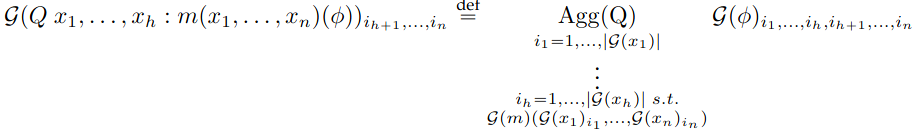
\includegraphics[width=\textwidth]{ltn5.png}
\end{block}
\end{frame}

\begin{frame}
  \frametitle{Guarded quantification}
  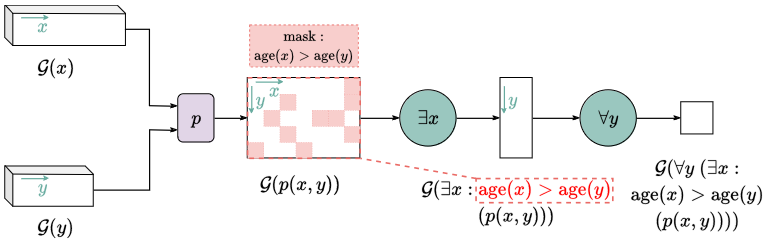
\includegraphics[width=\textwidth]{ltn6.png}
\end{frame}

% Slide: Machine Learning Setup in Fuzzy Logic
\begin{frame}
\frametitle{Where Do We Go From Here?}
\begin{block}{Towards a Machine Learning Setup}
\begin{itemize}
    \item Up to now, we have explored aspects of fuzzy logic.
    \item Moving forward, we transition to a machine learning setup:
    \begin{itemize}
        \item Objects are represented by points in a feature space.
        \item Functions and predicates become learnable entities.
    \end{itemize}
    \item Some examples...
\end{itemize}
\end{block}
\end{frame}

% Slide: Incorporating Knowledge through Grounding
\begin{frame}
\frametitle{Incorporating Knowledge through Grounding}
\begin{block}{Fixed Grounding of Symbols}
Knowledge can be strictly incorporated by fixing the grounding of symbols. For example:
\begin{itemize}
    \item A constant \( c \) denotes an object with features \(
      \mathbf{v}_c \in \mathbb{R}^n \), grounding \( \G(c) =
      \mathbf{v}_c \)
    \item Training data with \( n \) items (e.g., images) as \( n \)
      constants and their groundings
\end{itemize}
\end{block}

\begin{block}{Example Groundings}
For the MNIST dataset:
\begin{itemize}
    \item Groundings represented by constants:
      $\G(\text{img}_1)=$
\includegraphics[width=.03\textwidth]{8.png},
      $\G(\text{img}_2)=$
\includegraphics[width=.03\textwidth]{9.png},
      $\G(\text{img}_3)=$
\includegraphics[width=.03\textwidth]{2.png}
\end{itemize}
\end{block}
\end{frame}

% Slide: Incorporating Knowledge through Grounding
\begin{frame}
\frametitle{Incorporating Knowledge through Grounding}
\begin{block}{Grounding Functions and Predicates}
\begin{itemize}
    \item Binary predicate \( \text{sim} \) for similarity, grounded
      as a cosine similarity function
    \item Output layer of a neural network as a softmax function,
      ensuring \( \sum_i P(x, i) = 1 \)
    \item Transposition function example: \(
      \G(\text{transp}(\text{img}_1)) = \)
      
\includegraphics[width=.03\textwidth, angle=90]{8.png}
\end{itemize}
\end{block}
\end{frame}

% Slide 1: Parametric Definition of Grounding for Symbols
\begin{frame}
\frametitle{Parametric Definition of Grounding for Symbols}
\begin{block}{Grounding via Learning}
The grounding of a symbol \( \sigma \) is obtained by learning a set of real-valued parameters \( \theta_\sigma \), denoted as \( \G(\sigma) = \G(\sigma | \theta_\sigma) \).
\end{block}

\begin{block}{Parametric Grounding Examples}
\begin{itemize}
    \item \textbf{Word Embedding}: For words \( w_i \) in a vocabulary \( W \), their groundings \( \G(w_i | \theta_{\text{emb}}) \) are defined w.r.t. embedding parameters \( \theta_{\text{emb}} \).
    \item \textbf{Linear Functions}: A linear function symbol \( f \) can have grounding \( \G(f | \theta_f) \) with parameters \( \theta_f = (A_f, b_f) \).
\end{itemize}
\end{block}
\end{frame}

% Slide 2: Grounding of Predicate Symbols
\begin{frame}
\frametitle{Grounding of Predicate Symbols}
\begin{block}{Neural Networks as Grounding Functions}
The grounding of a predicate symbol can be represented by a neural network \( N \) with parameters \( \theta_N \).
\end{block}

\begin{block}{Example: Image Classification}
\begin{itemize}
    \item Neural network \( N \) classifies images into classes (e.g., cat, dog, horse) with output vector \( y \in [0, 1]^n \).
    \item Probability that image \( v \) belongs to class \( c \): \( y_c = N(v | \theta_N)_c \).
    \item Unary predicate symbols like \( \text{cat}(v) \), \( \text{dog}(v) \), \( \text{horse}(v) \) are grounded as \( \G(\text{cat}(v)) = N(v | \theta_N)_{\text{cat}}, G(\text{dog}(v)) = N(v | \theta_N)_{\text{dog}}, \ldots \)
\end{itemize}
\end{block}
\end{frame}

% Slide: Factual Propositions in Real Logic
\begin{frame}
\frametitle{Factual Propositions and Supervised Learning}
\begin{block}{Knowledge of Domain Properties}
Factual knowledge about domain properties is represented by logical propositions. For instance:
\begin{itemize}
    \item \( \text{nine}(\text{img}_1) \), \( \text{eight}(\text{img}_2) \), \( \ldots \), \( \text{two}(\text{img}_n) \) represent known classifications of images
\end{itemize}
\end{block}

\begin{block}{Supervised Learning in Real Logic}
Supervised learning using labelled data:
\begin{itemize}
    \item Grounding definitions combined with factual propositions specify training examples.
    \item For example, \( \G(\text{img}_1) \) is defined alongside propositions \( \text{nine}(\text{img}_1) \) and \( \neg\text{eight}(\text{img}_1) \) to represent labelled data.
\end{itemize}
\end{block}
\end{frame}


\begin{frame}
\frametitle{Semi-supervised and relational Learning}
\begin{block}{Semi-supervision and Relational Learning}
\begin{itemize}
    \item Semi-supervision expressed naturally with disjunctions, e.g., \( \text{eight}(\text{img}_1) \lor \text{nine}(\text{img}_1) \).
    \item Relational learning relates multiple objects, e.g., \( \text{nine}(\text{img}_1) \Rightarrow \neg\text{nine}(\text{img}_2) \).
\end{itemize}
\end{block}

\end{frame}

% Slide 1: Generalized Propositions in Real Logic
\begin{frame}
\frametitle{Generalized Propositions}
\begin{block}{General Knowledge Representation}
General knowledge about objects in domains can be specified using first-order logic formulas with quantified variables, allowing for constraints on groundings that hold for all objects within a domain.
\end{block}

\begin{block}{Use Cases in Machine Learning}
This form of knowledge representation is particularly useful in semi-supervised and unsupervised learning settings, where there is no specific knowledge about individual instances.
\end{block}
\end{frame}

% Slide 2: Examples of Generalized Propositions
\begin{frame}
\frametitle{Examples of Generalized Propositions}
\begin{block}{Multi-label Classification with Constraints}
For example, the constraint that if an instance is labeled with
$l_1,...,l_k$ it should also be labeled with $l_{k+1}$:
\[ \forall x (l_1(x) \land \ldots \land l_k(x) \Rightarrow l_{k+1}(x)) \]
\end{block}

\begin{block}{Statistical Relational Learning}
In statistical relational learning, soft constraints relate the labels
of associated examples. For instance:
\[ \forall x,y ((\text{smokes}(x) \land \text{friend}(x, y))
  \Rightarrow \text{smokes}(y)) \]
This encodes the soft constraint that friends of smokers are likely
smokers as well.
\end{block}
\end{frame}

% Slide 1: Components of a Real Logic Knowledge-Base
\begin{frame}
\frametitle{Components of a Real Logic Knowledge-Base}
\begin{block}{Knowledge-Base Components}
A Real Logic knowledge-base consists of:
\begin{enumerate}
    \item Knowledge about the grounding of symbols: domains, constants, variables, functions, and predicate symbols.
    \item A set of closed logical formulas for factual propositions and general knowledge.
    \item Operators and hyperparameters for formula evaluation.
\end{enumerate}
\end{block}

\begin{block}{Formal Definition of a Theory/Knowledge-Base}
\begin{itemize}
    \item Defined as a triple \( T = \langle K, \G(\cdot | \theta), \Theta \rangle \).
    \item \( K \): Set of closed first-order logic formulas.
    \item \( \G(\cdot | \theta) \): Parametric grounding for all symbols and logical operators.
    \item \( \Theta \): Hypothesis space for parameters associated with each symbol.
\end{itemize}
\end{block}
\end{frame}

% Slide 2: Learning and Reasoning in Real Logic Theory
\begin{frame}
\frametitle{Learning and Reasoning in Real Logic Theory}
\begin{block}{Grounded Theory and Parameter Optimization}
Learning and reasoning involve finding parameter values that maximize
the satisfaction of formulas in \( K \). A grounded theory \( \langle
K, \G_\theta \rangle \) refers to a Real Logic theory with a specific
set of learned parameter values.
\end{block}

\begin{block}{Satisfiability and Optimization Problem}
\begin{itemize}
    \item Similar to the weighted MAX-SAT problem with weights given by fuzzy truth-values derived from parameter values.
    \item Satisfiability for a theory \( T = \langle K, \G_\theta
      \rangle \) with respect to an aggregating operator \(
      \text{SatAgg} \) is defined as \( \text{SatAgg}_{\phi \in K}
      \G_\theta(\phi)) \)
\end{itemize}
\end{block}
\end{frame}

% Slide 1: Learning in Real Logic Theory
\begin{frame}
\frametitle{Learning in Real Logic Theory}
\begin{block}{Learning Process}
Given a Real Logic theory \( T = (K, G(\cdot | \theta), \Theta) \), learning is the process of finding parameter values \( \theta^* \) that maximize the satisfiability of \( T \) with respect to a given aggregator:
\[ \theta^* = \underset{\theta \in \Theta}{\text{argmax}} \, \underset{\phi \in K}{\text{SatAgg}}\G_\theta(\phi) \]
\end{block}

\begin{block}{Applications in Machine Learning}
\begin{itemize}
    \item Learning the grounding of constants is analogous to learning embeddings.
    \item Learning the grounding of functions is similar to generative modeling or regression tasks.
    \item Learning the grounding of predicates is akin to classification tasks.
\end{itemize}
\end{block}
\end{frame}

% Slide 2: Regularization in Learning
\begin{frame}
\frametitle{Regularization in Learning}
\begin{block}{Regularized Learning}
Incorporating regularization into the learning process imposes preferences on the hypothesis space \( \Theta \), often favoring smaller parameter values:
\[ \theta^* = \underset{\theta \in \Theta}{\text{argmax}} \left( \underset{\phi \in K}{\text{SatAgg}}\G_\theta(\phi)  - \lambda R(\theta) \right) \]
where \( \lambda \in \mathbb{R}_+ \) is the regularization parameter and \( R \) is a regularization function (e.g., L1 or L2 regularization).
\end{block}

\begin{block}{Generalization and Extrapolation}
\begin{itemize}
    \item LTN can generalize to new, unseen data using knowledge from previous groundings.
    \item Trained predicates can be re-used for querying formulas with new individuals from a domain.
\end{itemize}
\end{block}
\end{frame}

\begin{frame}
\frametitle{Query Answering and Truth Queries}
\begin{block}{Grounded Theory \( T = (K, \G_\theta) \)}
Query answering determines the truth-value of facts, which are real numbers in the interval [0,1].
\end{block}

\begin{block}{Truth Queries}
\begin{itemize}
    \item Any formula can be a truth query.
    \item The answer is the truth value obtained by computing the grounding: \( \G_\theta(\phi) \).
    \item If \( \phi \) has free variables \( x_1, \ldots, x_n \), the answer is a tensor of order \( n \).
\end{itemize}
\end{block}

\begin{block}{Value Queries}
\begin{itemize}
    \item Any term can be a value query, with the answer as a tensor of real numbers: \( \G_\theta(t) \).
    \item These queries allow inspection of how constants or terms are embedded in the manifold.
\end{itemize}
\end{block}
\end{frame}

% Slide 2: Generalization Queries in Grounded Theory
\begin{frame}
\frametitle{Generalization Queries in Grounded Theory}
\begin{block}{Generalization Truth Queries}
\begin{itemize}
    \item Used to determine truth-values for new, unseen objects in a domain.
    \item The query \( (\phi(x), U) \) evaluates \( \phi \) with free variable \( x \) on a new set \( U \) of examples.
    \item Results in a vector of truth-values for the evaluation of \( \phi \) on new data.
\end{itemize}
\end{block}

\begin{block}{Generalization Value Queries}
\begin{itemize}
    \item Similar to generalization truth queries but evaluate a term \( t(x) \) on new data \( U \).
    \item The result is a vector of values for the evaluation of a trained model on a regression task using test data \( U \).
\end{itemize}
\end{block}
\end{frame}

\begin{frame}
\frametitle{Reasoning from the logic perspective}
\begin{block}{Reasoning in Logic}
Reasoning is verifying if a formula is a logical consequence of a set
of formulas, either semantically via model theory (\(\models\)) or
syntactically via proof theory (\(\vdash\)).
\end{block}

\begin{block}{Fuzzy Logical Consequence}
  In fuzzy logic, a formula \(\phi\) is a logical consequence of a set
  of formulas \(\Gamma\) (\(\Gamma | \models \phi\)) if, for every
  fuzzy interpretation \(f\), \(\phi\) is true whenever all formulas
  in \(\Gamma\) are true.
\end{block}

\begin{block}{Practical Challenges in Real Logic}
Direct application of fuzzy logical consequence is impractical in Real
Logic, as satisfiability levels of grounded theories are rarely $1$.
\end{block}
\end{frame}

% Slide 2: Logical Consequence in Real Logic
\begin{frame}
\frametitle{Logical Consequence in Real Logic}
\begin{block}{Adapted Definition for Real Logic}
\begin{itemize}
    \item An interval \([q, 1]\) with \( \frac{1}{2} < q \leq 1\) is used, where a formula is true if its truth-value is within this interval.
\end{itemize}
\end{block}

\begin{block}{Definition of Logical Consequence}
\begin{itemize}
\item A closed formula \(\phi\) is a logical consequence of a
  knowledge-base \((K, \G(\cdot | \theta), \Theta)\), denoted
  \((K, \G(\cdot | \theta), \Theta) | \models_q \phi\), if for every
  grounded theory \(\langle K, \G_\theta \rangle\),
  \(\G_\theta(\phi) \geq q\) whenever
  \(\text{SatAgg}(K, \G_\theta) \geq q\).
\end{itemize}
\end{block}
\end{frame}

%Reasoning Option 1 - Querying after Learning
\begin{frame}
\frametitle{Reasoning Option 1: Querying after Learning}
\begin{block}{Approach}
This method involves approximate logical inference by considering only the grounded theories that maximally satisfy \( (K, \G(\cdot | \theta), \Theta) \).
\end{block}

\begin{block}{Brave Logical Consequence}
A formula \( \phi \) is considered a brave logical consequence of a Real Logic knowledge-base \( (K, \G(\cdot | \theta), \Theta) \) if \( \G_{\theta^*}(\phi) \geq q \) for all optimal \( \theta^* \) that maximize \( \text{SatAgg}(K, \G_\theta) \) and ensure \( \text{SatAgg}(K, \G_{\theta^*}) \geq q \).
\end{block}

\begin{block}{Challenges}
\begin{itemize}
    \item The approach may not fully represent all optimal or close-to-optimal groundings.
    \item Multiple optimizations might not reach different optima in the search space.
\end{itemize}
\end{block}
\end{frame}

% Slide: Reasoning Option 2 - Proof by Refutation
\begin{frame}
\frametitle{Reasoning Option 2: Proof by Refutation}
\begin{block}{Refutation as Reasoning}
Reasoning by refutation searches for a counter-example to disprove a logical consequence.
\end{block}

\begin{block}{Dual Problem}
\begin{itemize}
    \item Traditional approach: For all \( \theta \in \Theta \), if \( G_\theta(K) \geq q \) then \( G_\theta(\phi) \geq q \).
    \item Refutation approach: Exists \( \theta \in \Theta \) such that \( G_\theta(K) \geq q \) and \( G_\theta(\phi) < q \).
    \item If true, a counterexample exists, and the logical consequence does not hold.
\end{itemize}
\end{block}

\begin{block}{Implementation}
\begin{itemize}
    \item The objective is to minimize \( G_\theta(\phi) \) while imposing a constraint against \( G_\theta(K) < q \).
\end{itemize}
\end{block}
\end{frame}

\begin{frame}
\frametitle{Defining the Penalty Function}
\begin{block}{Penalty Function for Refutation}
\begin{itemize}
    \item Define a penalty function: 
    \[ \text{penalty}(G_\theta, q) = 
       \begin{cases} 
       c & \text{if } G_\theta(K) < q, \\
       0 & \text{otherwise},
       \end{cases} \]
    where \( c > 1 \).
\end{itemize}
\end{block}
\end{frame}

% Slide 2: Optimization and Logical Consequence
\begin{frame}
\frametitle{Optimization and Logical Consequence}
\begin{block}{Optimization Objective}
\begin{itemize}
    \item Objective is to find \( G^* \) minimizing \( G_\theta(\phi) \) plus penalty, given by:
    \[ G^* = \text{argmin}_{G_\theta} \left( G_\theta(\phi) + \text{penalty}(G_\theta, q) \right) \]
\end{itemize}
\end{block}

\begin{block}{Determining Logical Consequence}
\begin{itemize}
    \item If \( G^*(K) < q \): Then for all \( G_\theta \), \( G_\theta(K) < q \) and \( (K, G(\cdot | \theta), \Theta) \models_q \phi \).
    \item If \( G^*(K) \geq q \) and \( G^*(\phi) \geq q \): for all
      $G_\theta$ with $G_\theta(K) \geq q$: $G_\theta(\phi) \geq
      G^*(\phi) \geq q$, therefore $(K, G(\cdot | \theta), \Theta)
      \models_q \phi$.
    \item If \( G^*(K) \geq q \) and \( G^*(\phi) < q \): Logical consequence does not hold.
\end{itemize}
\end{block}
\end{frame}

% Slide: Optimization Challenges and Solutions
\begin{frame}
\frametitle{Optimization Challenges and Solutions}
\begin{block}{Challenge with refutation}
\begin{itemize}
    \item Direct use of previous equation for gradient descent is
      impractical due to null derivatives.
\end{itemize}
\end{block}

\begin{block}{Approximating the Penalty Function}
\begin{itemize}
    \item A soft constraint is proposed to approximate the penalty function:
    \[ \text{elu}(\alpha, \beta(q - G_\theta(K))) = 
    \begin{cases} 
    \beta(q - G_\theta(K)) & \text{if } G_\theta(K) \leq q, \\
    \alpha(\exp(q-G_\theta(K)) - 1) & \text{otherwise},
    \end{cases} \]
    \item Where \( \alpha \geq 0 \) and \( \beta \geq 0 \) act as hyper-parameters.
\end{itemize}
\end{block}
\end{frame}

\begin{frame}
  \frametitle{Optimization objective}
  \begin{block}{Optimization Objective}
    \begin{itemize}
    \item The approximate objective function is defined as:
      \[ G^* = \text{argmin}_{G_\theta} \left( G_\theta(\phi) +
          \text{elu}(\alpha, \beta(q - G_\theta(K))) \right) \]
    \item This formulation enables the use of gradient descent
      algorithms.
    \end{itemize}
  \end{block}
\end{frame}

% Slide 1: Introduction to Binary Classification with LTN
\begin{frame}
\frametitle{Example: Binary Classification with LTN}
\begin{block}{Task Overview}
Binary classification in \( \mathbb{R}^2 \) using LTN with positive
and negative examples.
\end{block}

\begin{block}{Language and Grounding}
\begin{itemize}
    \item \textbf{Domains:} Points (representing examples).
    \item \textbf{Variables:} \( x^+ \) for positive, \( x^- \) for
      negative, and \( x \) for all examples.
    \item \textbf{Predicates:} \( A(x) \) as the trainable classifier.
    \item \textbf{Axioms:} \( \forall x^+ A(x^+), \forall x^- \neg A(x^-) \).
\end{itemize}
\end{block}
\end{frame}

\begin{frame}
  \frametitle{Grounding}
  \begin{block}{Grounding Setup}
    \begin{itemize}
    \item Domain of points: \( G(\text{points}) = \mathbb{R}^2 \).
    \item Examples sequence: \( G(x) \) is a sequence of \( m \) points in \( \mathbb{R}^{m \times 2} \).
    \item Positive examples \( G(x^+) \): Points within Euclidean
      distance \( < 0.09 \) to \( (0.5, 0.5) \)
      \begin{itemize}
      \item \( G(x^+) \) denotes training examples closer than $0.09$ to center \( (0.5, 0.5) \)
      \end{itemize}
    \item Negative examples \( G(x^-) \): Points with Euclidean distance \( \geq 0.09 \) to \( (0.5, 0.5) \)
\end{itemize}
\end{block}
\end{frame}


\begin{frame}
  \frametitle{Grounding}
  \begin{block}{Classifier Grounding}
    \begin{itemize}
    \item Trainable classifier \( A(x) \) grounded as \( G(A |
      \theta): x \mapsto \text{sigmoid}(\text{MLP}_\theta(x)) \)
      where MLP is a Multilayer Perceptron.
    \end{itemize}
  \end{block}
\end{frame}

\begin{frame}
  \frametitle{Binary Classification}
  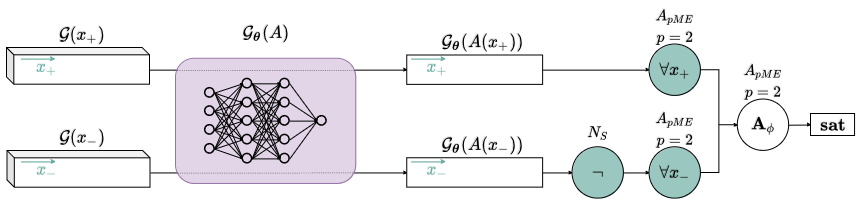
\includegraphics[width=\textwidth]{ex1.png}
\end{frame}


% Slide 2: Learning Process in LTN
\begin{frame}
  \frametitle{Learning Process in LTN}
  \begin{block}{Objective and Loss Function}
    Objective function defined by
    \( \text{argmax}_{\theta \in \Theta} \text{SatAgg}(\{\phi \in K\},
    G_{\theta, x \leftarrow D}(\phi)) \) with a custom loss function
    \begin{itemize}
    \item $G_{x \leftarrow D}$ means that the variable $x$ is grounded
      with the data $D$ ($G(x) := D$ when grounding $x$)
    \end{itemize}
  \end{block}
\end{frame}

\begin{frame}
  \frametitle{Loss function}
  \begin{block}{Loss Function for Optimization}
    The loss function used by the optimizer is defined as:
    \[ L = \left( 1 - \text{SatAgg} \left( \{\phi \in K\}, G_{\theta, x
            \in B}(\phi) \right) \right) \]
  \end{block}
  \begin{block}{Explanation}
    \begin{itemize}
    \item \(L\): The loss function.
    \item \(\text{SatAgg}\): The satisfaction aggregator function, aggregating the satisfaction levels of formulas in the knowledge base \(K\).
    \item \(G_{\theta, x \leftarrow B}(\phi)\): The grounding of the
      formula \(\phi\) for a mini-batch \(B\) of examples,
      parameterized by \(\theta\).
    \item The loss function aims to minimize the difference between
      perfect satisfaction and the actual aggregated satisfaction
      of the formulas for the given batch.
\end{itemize}
\end{block}  
\end{frame}

\begin{frame}
  \frametitle{Hyper-Parameters and satisfiability}
  \begin{itemize}
  \item Choice of fuzzy logic operator semantics.
  \item Value of the exponent \( p \) in generalized mean.
  \item Formula aggregator function.
  \end{itemize}
  \begin{block}{Using Stable Product Configuration}
    Approximating connectives and quantifiers with the stable product
    configuration and \(p = 2\) for $A_{pME}$:
    \begin{itemize}
    \item Applies to both the occurrence of $A_{pME}$ and the formula aggregator function
    \end{itemize}
  \end{block}
\end{frame}
  
\begin{frame}
  \frametitle{Hyper-Parameters and satisfiability}
\begin{block}{Satisfaction Equation}
  The satisfaction equation is given by:
  \tiny
\begin{align*}
\text{SatAgg}(\{\phi \in K\}, G_\theta(\phi)) = 1 &- \frac{1}{2} \left[ \left( 1 - \frac{1}{|G(x^+)|} \sum_{v \in G(x^+)} \left(1 - \text{sigmoid}(\text{MLP}_\theta(v))\right)^2 \right)^2 \right. \\
&+ \left. \left( 1 - \frac{1}{|G(x^-)|} \sum_{v \in G(x^-)} \left(\text{sigmoid}(\text{MLP}_\theta(v))\right)^2 \right)^2 \right]
\end{align*}
\end{block}
\end{frame}

% Slide 3: Results Visualization
\begin{frame}
\frametitle{Results Visualization}
\begin{block}{Classification Accuracy and Satisfaction Level}
\begin{itemize}
    \item 100 data points sampled uniformly from \( \mathbb{R}^2 \).
    \item Split into training and testing sets, trained over 1000 epochs.
\end{itemize}
\end{block}

\begin{figure}
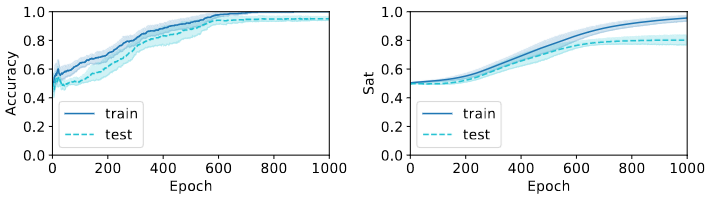
\includegraphics[width=\textwidth]{ltn1000.png}
\caption{Classification accuracy and satisfaction level over 1000 epochs.}
\end{figure}
\end{frame}


\end{document}


%%% Local Variables:
%%% mode: latex
%%% coding: utf-8
%%% TeX-master: t
%%% eval: (TeX-run-style-hooks "beamer")
%%% End:
